\documentclass[11pt,a4paper]{article}

\usepackage[a4paper,margin=18mm]{geometry}
\usepackage[T1]{fontenc}
\usepackage[utf8]{inputenc}
\usepackage{lmodern,microtype,parskip,enumitem,booktabs,tabularx,array,longtable}
\usepackage{xcolor,hyperref,tikz,pgfplots,tcolorbox,listings,titlesec,fancyhdr}
\usepackage{amsmath,amssymb,caption,float}
\usetikzlibrary{arrows.meta,positioning,calc}
\pgfplotsset{compat=1.18}

\definecolor{navy}{HTML}{17324D}
\definecolor{blue}{HTML}{2C6EAA}
\definecolor{teal}{HTML}{2A9D8F}
\definecolor{gold}{HTML}{E9C46A}
\definecolor{orange}{HTML}{F4A261}
\definecolor{red}{HTML}{E76F51}
\definecolor{lightblue}{HTML}{EAF4FB}
\definecolor{lightgray}{HTML}{F4F6F8}
\definecolor{darkgray}{HTML}{495057}

\hypersetup{colorlinks=true,linkcolor=navy,urlcolor=blue}
\setlength{\headheight}{14pt}
\emergencystretch=2em
\pagestyle{fancy}
\fancyhf{}
\lhead{\textcolor{darkgray}{Hanabi-CK}}
\rhead{\textcolor{darkgray}{Harness guide}}
\cfoot{\thepage}
\renewcommand{\headrulewidth}{0.2pt}

\titleformat{\section}{\Large\bfseries\color{navy}}{\thesection.}{0.6em}{}
\titleformat{\subsection}{\large\bfseries\color{navy}}{\thesubsection}{0.6em}{}

\newcolumntype{Y}{>{\raggedright\arraybackslash}X}
\newcolumntype{C}{>{\centering\arraybackslash}X}
\lstset{
  basicstyle=\ttfamily\small,
  backgroundcolor=\color{lightgray},
  frame=single,
  breaklines=true,
  columns=fullflexible,
  showstringspaces=false
}
\newtcolorbox{callout}[1][]{
  colback=lightblue,colframe=blue,boxrule=0.8pt,arc=2mm,
  title=#1,fonttitle=\bfseries,left=3mm,right=3mm,top=2mm,bottom=2mm
}
\newtcolorbox{warningbox}[1][]{
  colback=orange!10,colframe=orange!90!black,boxrule=0.8pt,arc=2mm,
  title=#1,fonttitle=\bfseries,left=3mm,right=3mm,top=2mm,bottom=2mm
}

\begin{document}

\begin{titlepage}
\centering
\vspace*{18mm}
{\Huge\bfseries\color{navy} Hanabi-CK\par}
\vspace{3mm}
{\LARGE A practical harness for testing common knowledge and coordination in LLM agents\par}
\vspace{8mm}
{\large Illustrated guide to the research question, system design, failure modes, fixes, and current experiments\par}
\vspace{14mm}

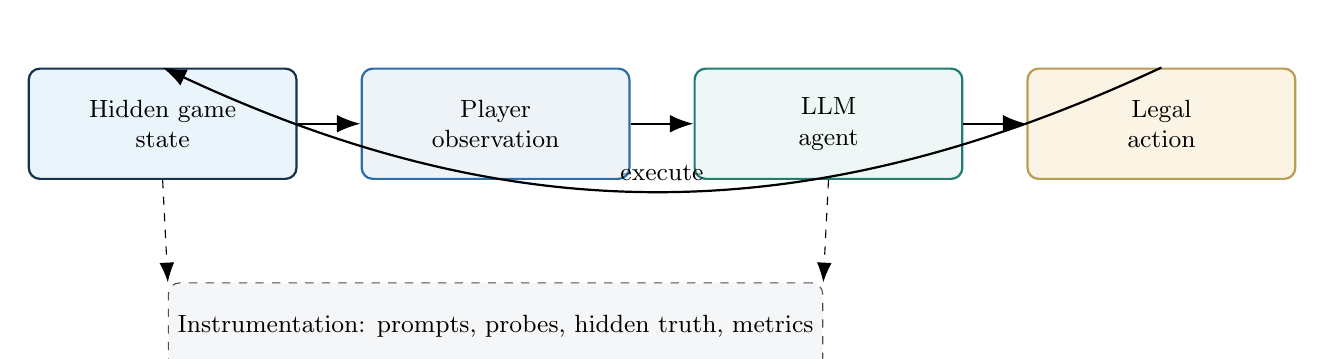
\begin{tikzpicture}[node distance=9mm and 8mm,every node/.style={font=\small,align=center}]
\node[draw=navy,thick,rounded corners,fill=lightblue,minimum width=34mm,minimum height=14mm] (state) {Hidden game\\state};
\node[draw=blue,thick,rounded corners,fill=blue!8,right=of state,minimum width=34mm,minimum height=14mm] (obs) {Player\\observation};
\node[draw=teal!80!black,thick,rounded corners,fill=teal!8,right=of obs,minimum width=34mm,minimum height=14mm] (agent) {LLM\\agent};
\node[draw=gold!80!black,thick,rounded corners,fill=gold!18,right=of agent,minimum width=34mm,minimum height=14mm] (act) {Legal\\action};
\draw[-{Latex[length=3mm]},thick] (state)--(obs);
\draw[-{Latex[length=3mm]},thick] (obs)--(agent);
\draw[-{Latex[length=3mm]},thick] (agent)--(act);
\draw[-{Latex[length=3mm]},thick,bend left=25] (act.north) to node[above]{execute} (state.north);
\node[draw=darkgray,dashed,rounded corners,fill=lightgray,below=13mm of obs,minimum width=68mm,minimum height=11mm] (log) {Instrumentation: prompts, probes, hidden truth, metrics};
\draw[-{Latex[length=2.5mm]},dashed] (state.south)--(log.north west);
\draw[-{Latex[length=2.5mm]},dashed] (agent.south)--(log.north east);
\end{tikzpicture}

\vfill
\begin{callout}[One-sentence goal]
We want to know whether an LLM can use not only what it knows, but what it believes its partner knows, and whether that shared epistemic structure changes coordinated behavior.
\end{callout}
\vspace{5mm}
\textbf{Repository:} \url{https://github.com/pabloloyola/hanabi-ck}
\end{titlepage}

\tableofcontents
\newpage

\section{What are we testing?}

Hanabi is a cooperative card game with hidden self-information: each player can see the other player's cards but not their own. Players cannot freely explain a plan. Communication occurs through constrained hints and through actions.

\begin{callout}[Research question]
Can LLM agents establish, recognize, exploit, and recover common knowledge in a cooperative partially observable environment?
\end{callout}

The progression we care about is:
\begin{itemize}[leftmargin=1.5em]
\item I know the convention.
\item I know my partner knows the convention.
\item I know my partner knows that I know it.
\item The convention is treated as public/common knowledge.
\end{itemize}

\subsection{Starter convention}

\begin{callout}[Convention]
If a player gives a rank hint that touches the receiver's newest card, the receiver should interpret that newest card as intended to be played as soon as it is safe to do so.
\end{callout}

\subsection{Epistemic ladder}

\begin{table}[H]
\centering
\small
\begin{tabularx}{\textwidth}{>{\bfseries}p{25mm}YY}
\toprule
Condition & Information supplied & Purpose \\
\midrule
CK0 & No convention & Baseline \\
CK1 private & One designated player privately gets it & Asymmetric knowledge \\
CK2 shared & Both privately get it; no meta-information & Shared fact without mutual assurance \\
CK3 mutual & Both get it and are told everyone got it & Finite mutual knowledge \\
CK$\infty$ common & Public/common-knowledge declaration & Strongest public framing \\
\bottomrule
\end{tabularx}
\end{table}

\section{How the harness works}

\begin{figure}[H]
\centering
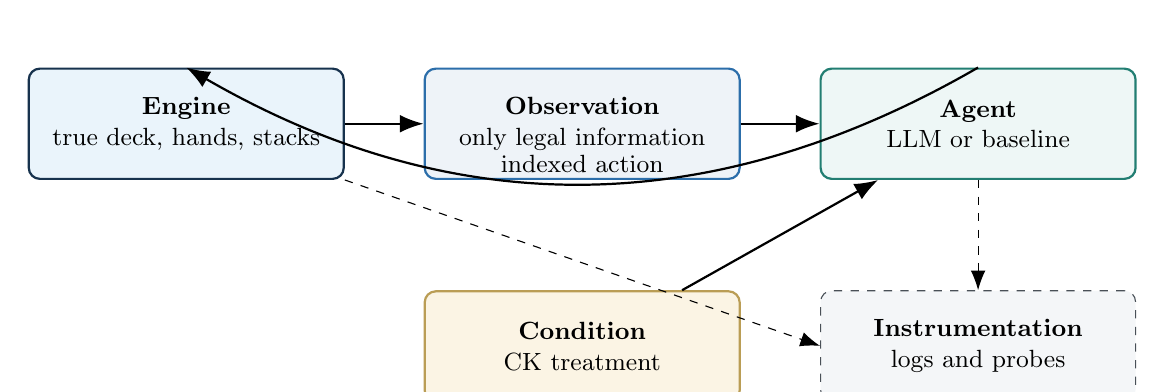
\begin{tikzpicture}[node distance=10mm and 10mm,every node/.style={font=\small,align=center}]
\node[draw=navy,thick,rounded corners,fill=lightblue,minimum width=40mm,minimum height=14mm] (engine) {\textbf{Engine}\\true deck, hands, stacks};
\node[draw=blue,thick,rounded corners,fill=blue!8,right=of engine,minimum width=40mm,minimum height=14mm] (obs) {\textbf{Observation}\\only legal information};
\node[draw=teal!80!black,thick,rounded corners,fill=teal!8,right=of obs,minimum width=40mm,minimum height=14mm] (agent) {\textbf{Agent}\\LLM or baseline};
\node[draw=gold!80!black,thick,rounded corners,fill=gold!18,below=14mm of obs,minimum width=40mm,minimum height=14mm] (cond) {\textbf{Condition}\\CK treatment};
\node[draw=darkgray,dashed,rounded corners,fill=lightgray,below=14mm of agent,minimum width=40mm,minimum height=14mm] (metrics) {\textbf{Instrumentation}\\logs and probes};
\draw[-{Latex[length=3mm]},thick] (engine)--(obs);
\draw[-{Latex[length=3mm]},thick] (obs)--(agent);
\draw[-{Latex[length=3mm]},thick] (cond)--(agent);
\draw[-{Latex[length=3mm]},thick,bend left=30] (agent.north) to node[above]{indexed action} (engine.north);
\draw[-{Latex[length=2.5mm]},dashed] (engine.south east)--(metrics.west);
\draw[-{Latex[length=2.5mm]},dashed] (agent.south)--(metrics.north);
\end{tikzpicture}
\caption{The engine owns truth; the agent receives only the allowed observation plus the experimental treatment.}
\end{figure}

A single turn is:
\begin{enumerate}
\item Build \texttt{PlayerObservation}.
\item Inject the CK treatment.
\item Enumerate legal actions and assign each an \texttt{action\_index}.
\item Ask the model to return only \texttt{\{"action\_index": N\}}.
\item Map the index to the legal Hanabi action and execute it.
\item Log the player-visible view and researcher-only truth.
\end{enumerate}

\begin{lstlisting}
legal_actions = [
  {"action_index": 6,
   "action": {"type": "play", "card_index": 1}},
  {"action_index": 13,
   "action": {"type": "play", "card_index": 4}}
]

model_output = {"action_index": 13}
\end{lstlisting}

\begin{callout}[Why indexed actions?]
The old output schema could produce malformed hybrids, for example a play action carrying hint fields. Indexed selection removes formatting ambiguity without changing the strategic choice.
\end{callout}

\subsection{Visible versus hidden information}

\begin{table}[H]
\centering
\small
\begin{tabularx}{\textwidth}{YY}
\toprule
\textbf{Agent-visible} & \textbf{Researcher-only} \\
\midrule
Partner's actual hand & Acting player's hidden cards \\
Own hint-derived possibilities & True deck order \\
Public stacks, discards, tokens & Exact hidden identities \\
Public action history & Full ground truth \\
Derived safety from legal information & Outcome labels and diagnostics \\
\bottomrule
\end{tabularx}
\end{table}

\section{What do Hanabi moves look like?}

\begin{table}[H]
\centering
\small
\begin{tabularx}{\textwidth}{>{\bfseries}p{20mm}p{78mm}Y}
\toprule
Action & Example & Meaning \\
\midrule
Hint & \texttt{\{"type":"hint","target":1,"attribute":"rank","value":1\}} & Tell P1 which cards have rank 1. \\
Play & \texttt{\{"type":"play","card\_index":4\}} & Attempt to play own slot 4. \\
Discard & \texttt{\{"type":"discard","card\_index":0\}} & Discard own slot 0. \\
\bottomrule
\end{tabularx}
\end{table}

\subsection{Illustrated convention-sensitive hint}

\begin{figure}[H]
\centering
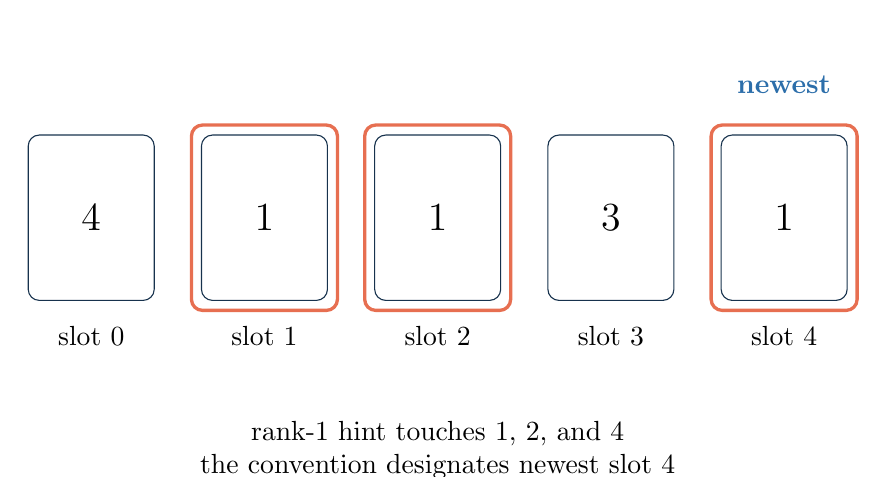
\begin{tikzpicture}[x=1cm,y=1cm]
\foreach \x/\idx/\rank in {0/0/4,2.2/1/1,4.4/2/1,6.6/3/3,8.8/4/1}{
  \node[draw=navy,rounded corners,minimum width=16mm,minimum height=21mm] at (\x,0) (c\idx) {\Large \rank};
  \node[below=2mm of c\idx] {slot \idx};
}
\node[above=4mm of c4,font=\bfseries\color{blue}] {newest};
\foreach \idx in {1,2,4}{
  \draw[red,very thick,rounded corners] ($(c\idx.north west)+(-0.12,0.12)$) rectangle ($(c\idx.south east)+(0.12,-0.12)$);
}
\node[below=14mm of c2,align=center] {rank-1 hint touches 1, 2, and 4\\the convention designates newest slot 4};
\end{tikzpicture}
\end{figure}

\subsection{Epistemic safety}

A play is counted as justified only when every identity still compatible with the player's legal information is playable:
\[
\mathrm{safe}(i)=1
\iff
\forall(c,r)\in K_i,\quad \mathrm{stack}[c]+1=r.
\]

\begin{lstlisting}
{
  "provably_playable_indices": [1, 2, 4],
  "provably_obsolete_indices": [],
  "play_safety": {
    "1": "provably_safe",
    "2": "provably_safe",
    "4": "provably_safe"
  }
}
\end{lstlisting}

\begin{warningbox}[Why this matters]
A physically successful move can still be epistemically unjustified. Score alone can reward luck, so the harness records physical success and epistemic safety separately.
\end{warningbox}

\section{Failures we encountered and how the harness changed}

\subsection{Timeouts}
The first local Qwen run could time out before turn 0. We increased timeouts, bounded generation, and made agent errors abort a research game instead of silently substituting a random move.

\subsection{The model answered in reasoning\_content}
LM Studio sometimes returned empty \texttt{message.content} while the structured JSON appeared in \texttt{message.reasoning\_content}. The parser now checks content first and falls back to reasoning content.

\subsection{Malformed action objects}
The original schema forced every response to include play and hint fields at once. We replaced this with \texttt{action\_index} selection.

\subsection{Hinted card interpreted as play-now}
Full-game traces showed the model sometimes played partially known cards. We added \texttt{provably\_playable\_indices} and explicitly separated intended from safe.

\subsection{Full-game score was too noisy}
Dozens of turns mixed convention use with hints, discards, risk taking, and lucky plays. We therefore introduced deterministic micro-Hanabi scenarios.

\section{One-step micro diagnostic}

The current scenario freezes the game after P0 gives a rank-1 hint. Slots 1, 2, and 4 are all provably playable; slot 4 is newest. The only special reason to choose slot 4 is the convention.

\begin{callout}[Primary behavioral metric]
\[
\texttt{newest\_selection\_rate}
=P(\text{play newest touched safe card}\mid\text{condition}).
\]
\end{callout}

A separate stateless shadow probe asks which candidate card the partner intended:
\begin{lstlisting}
{"intended_card_index": 4}
\end{lstlisting}
The probe is never fed back into the action context.

\subsection{Current 100-repetition result}

\begin{figure}[H]
\centering
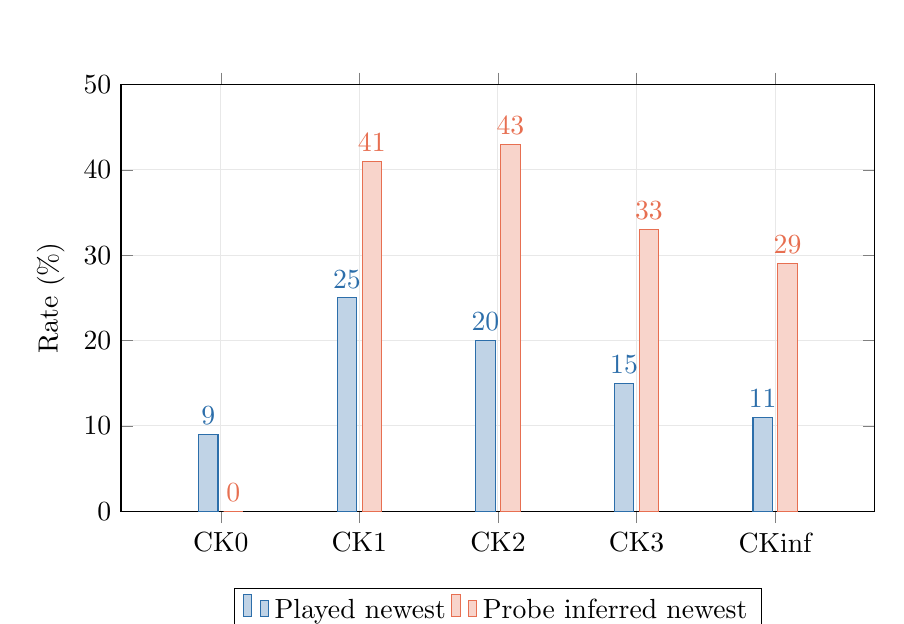
\begin{tikzpicture}
\begin{axis}[
ybar,bar width=7pt,width=.92\textwidth,height=7cm,
ymin=0,ymax=50,ylabel={Rate (\%)},
symbolic x coords={CK0,CK1,CK2,CK3,CKinf},xtick=data,
legend style={at={(0.5,-0.18)},anchor=north,legend columns=2},
nodes near coords,enlarge x limits=.18,grid=major,grid style={draw=gray!18}]
\addplot coordinates {(CK0,9) (CK1,25) (CK2,20) (CK3,15) (CKinf,11)};
\addplot coordinates {(CK0,0) (CK1,41) (CK2,43) (CK3,33) (CKinf,29)};
\legend{Played newest,Probe inferred newest}
\end{axis}
\end{tikzpicture}
\end{figure}

\begin{table}[H]
\centering
\small
\begin{tabularx}{\textwidth}{>{\bfseries}p{28mm}CCC}
\toprule
Condition & Played newest & Probe inferred newest & Recognition $-$ behavior \\
\midrule
CK0 & 9\% & 0\% & $-9$ pp \\
CK1 private & 25\% & 41\% & $+16$ pp \\
CK2 shared & 20\% & 43\% & $+23$ pp \\
CK3 mutual & 15\% & 33\% & $+18$ pp \\
CK$\infty$ common & 11\% & 29\% & $+18$ pp \\
\bottomrule
\end{tabularx}
\end{table}

The clean interpretation is that supplying the convention changes recognition and behavior relative to CK0, but the effect is not monotonic with stronger epistemic framing.

A useful methodological warning also emerged: CK1 and CK2 intentionally gave the receiver identical local wording, but outputs were not identical. The local model stack is therefore not perfectly deterministic even with a supplied seed.

\section{Latest reproducibility controls}

The micro runner now:
\begin{itemize}
\item randomizes condition order within each repetition;
\item pairs conditions using the same model seed and legal-action order;
\item hashes the exact action and probe request payloads;
\item reports Wilson intervals and paired condition transitions;
\item reports an explicit recognition-behavior gap;
\item labels the action/probe co-indexed statistic descriptively rather than as causal mediation.
\end{itemize}

\section{Two-agent sender to receiver diagnostic}

The next experiment tests both convention encoding and decoding. P0 is given the goal to communicate that P1 should play their newest card, but P0 may use only one legal Hanabi hint. The sender-facing goal deliberately avoids the numeric slot label so it cannot be mistaken for a rank value. The revised hand also removes rank 4 as a legal sender hint while preserving the rank-1 convention trigger on slots 1, 2, and 4. P1 then receives the observation caused by the actual hint and chooses an action.

\begin{figure}[H]
\centering
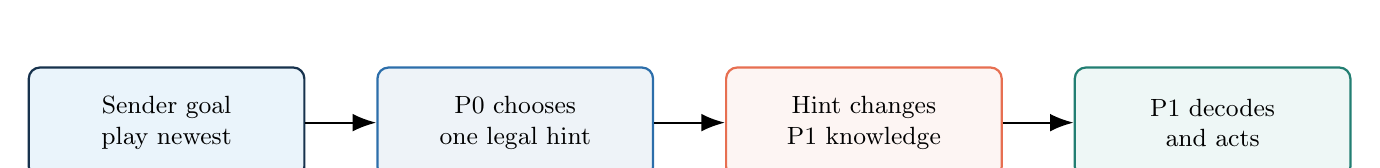
\begin{tikzpicture}[node distance=9mm and 9mm,every node/.style={font=\small,align=center}]
\node[draw=navy,thick,rounded corners,fill=lightblue,minimum width=35mm,minimum height=14mm] (goal) {Sender goal\\play newest};
\node[draw=blue,thick,rounded corners,fill=blue!8,right=of goal,minimum width=35mm,minimum height=14mm] (sender) {P0 chooses\\one legal hint};
\node[draw=red,thick,rounded corners,fill=red!7,right=of sender,minimum width=35mm,minimum height=14mm] (obs) {Hint changes\\P1 knowledge};
\node[draw=teal!80!black,thick,rounded corners,fill=teal!8,right=of obs,minimum width=35mm,minimum height=14mm] (recv) {P1 decodes\\and acts};
\draw[-{Latex[length=3mm]},thick] (goal)--(sender);
\draw[-{Latex[length=3mm]},thick] (sender)--(obs);
\draw[-{Latex[length=3mm]},thick] (obs)--(recv);
\end{tikzpicture}
\end{figure}

For the sender, each legal hint is additionally annotated with its deterministic
\texttt{touched\_indices}, which are derivable from the visible receiver hand.
This removes an unnecessary mechanical reasoning burden from the diagnostic.

This lets us ask:
\begin{itemize}
\item Does the sender choose the convention-triggering hint?
\item Does the receiver have enough epistemic reason to decode it?
\item Does the receiver play the intended newest card?
\item Do CK3/CK$\infty$ help more than CK1/CK2 when both agents participate?
\end{itemize}

\begin{lstlisting}[language=bash]
# Revised-scenario pilot first
uv run hanabi-ck micro-pair configs/micro_pair_pilot.yaml

# Scale only if sender convention use is healthy
uv run hanabi-ck micro-pair configs/micro_pair_newest.yaml
\end{lstlisting}

\section{What gets logged}

\begin{longtable}{>{\bfseries}p{50mm}p{105mm}}
\toprule
Field & Why it exists \\
\midrule
\endfirsthead
\toprule
Field & Why it exists \\
\midrule
\endhead
condition / repetition & Treatment and paired sample \\
private\_instruction\_hash & Exact epistemic prompt treatment \\
observation & Exact legal information shown to the agent \\
legal actions & Exact decision set \\
request\_payload\_hash & Verify byte-equivalent API requests where expected \\
raw / API response & Debug formatting, finish reason, token use \\
selected action & Behavioral outcome \\
epistemic safety & Separate justified play from luck \\
shadow probe & Measure inferred partner intention without feedback \\
researcher truth & Post-hoc correctness analysis hidden from the agent \\
\bottomrule
\end{longtable}

\subsection{Concrete logged example}

In CK0 repetition 0 of the 100-repetition run, the target was card 4. The action chose card 4, while the independent probe said card 1:
\begin{lstlisting}
selected_action: {"type": "play", "card_index": 4}
selected_newest_target: true
probe_intended_card_index: 1
probe_inferred_newest_target: false
\end{lstlisting}

\section{How to interpret future results}

\begin{table}[H]
\centering
\scriptsize
\begin{tabularx}{\textwidth}{p{40mm}YY}
\toprule
Pattern & Interpretation & Next check \\
\midrule
Probe rises, action does not & Recognition without operationalization & Policy bias and action prompt \\
Sender uses convention, receiver fails & Encoding works, decoding assumption is weak & CK depth and partner model \\
CK1/CK2 differ with identical request hashes & Infrastructure nondeterminism & Replicate and test server determinism \\
CK3/CK$\infty$ beat CK1/CK2 in pair harness & Mutual/public knowledge may help coordination & Repeat across scenarios/models/seats \\
Score rises while unsafe-play rate rises & Risk/luck rather than coordination & Use safety and micro diagnostics \\
\bottomrule
\end{tabularx}
\end{table}

\subsection{Near-term roadmap}
\begin{enumerate}
\item Rerun the one-step micro test with interleaved conditions and inspect CK1/CK2 request-hash matches.
\item Run the sender-receiver micro-pair experiment.
\item Add matched wording and placebo-public-statement controls.
\item Replicate with multiple models and both seat orders.
\item Return to full games and cross-play only after the micro mechanisms are stable.
\end{enumerate}

\section{Useful commands}

\begin{lstlisting}[language=bash]
uv run pytest

uv run hanabi-ck micro configs/micro_newest.yaml

uv run hanabi-ck micro-pair configs/micro_pair_newest.yaml

uv run hanabi-ck run configs/llm_debug.yaml
\end{lstlisting}

\section*{Evidence note}
The numerical results in this guide come from the 100-repetition \texttt{micro\_newest} summary. The interleaved-condition/request-hash controls and sender-receiver pair harness were implemented after that run and require fresh experiments.

\section*{Reference}
Bard, N. et al. (2020). \emph{The Hanabi Challenge: A New Frontier for AI Research}. Artificial Intelligence, 280, 103216.

\end{document}
